\documentclass[10pt]{standalone}
\usepackage{tikz}
\usepackage{lmodern}
\usepackage[T1]{fontenc}
\usepackage[utf8]{inputenc}
\usepackage{amsmath}
\usepackage{mathtools}
\usepackage{graphicx}
\usepackage{bbm}
\usepackage[margin=1in]{geometry}
\usepackage{caption}
\usepackage{subcaption}
\usepackage{float}
\usepackage{tikz}
\usetikzlibrary{ decorations.markings}
\usepackage[RPvoltages]{circuitikz}

\usetikzlibrary{decorations.pathreplacing,angles,quotes}

\usepackage{tikz,bm} % Useful for drawing plots

\usetikzlibrary{shapes.geometric, arrows}
\tikzstyle{process1} = [rectangle, draw = black, rounded corners, minimum width=0.8cm, minimum height=0.8cm, text centered, line width=0.5mm]
\tikzstyle{process2} = [rectangle, rounded corners, draw= red, minimum width=0.8cm, minimum height=0.8cm, text centered, line width=0.5mm]

\tikzstyle{process3} = [rectangle, draw = orange, rounded corners, minimum width=0.8cm, minimum height=0.8cm, text centered, line width=0.5mm]
\tikzstyle{legend} = [rectangle, minimum width=5cm, minimum height=2cm, , draw=black,fill=white, line width=1mm]
\tikzstyle{legend2} = [rectangle, minimum width=5cm, minimum height=3cm, , draw=black,fill=white, line width=1mm]
\tikzstyle{arrow} = [thick,->,>=stealth]
\usetikzlibrary{positioning}
\usetikzlibrary{calc}
\usepackage{circuitikz}


\usepackage{genealogytree}
\gtruselibrary{templates}
\usetikzlibrary{arrows.meta,positioning}
\usepackage[figurename=Figure]{caption} %
\usepackage{amsfonts} %
\usepackage{xcolor} %
\usepackage{enumitem}

\usetikzlibrary{shapes.multipart}

\title{Extract from Notes}

\date{}
\begin{document}
	
	\begin{minipage}{\linewidth}
		\centering
		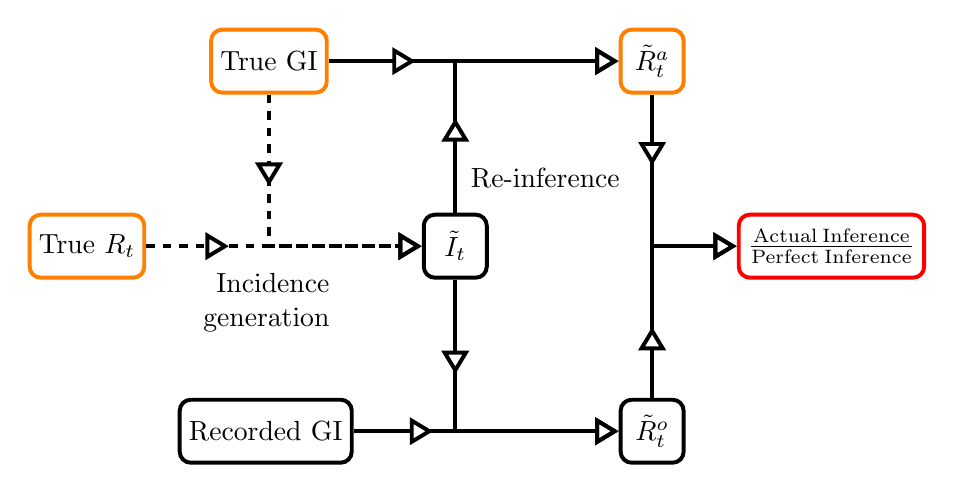
\begin{tikzpicture}[every text node part/.style={align=right}, decoration={markings, 
			mark= at position 0.3 with {\arrow{Triangle[open, scale=1.25, fill=white]}}}]
		
		\node (Rt) [process3] {True $R_t$};
		
		\node (GItrue) [process3,above right = 1.5cm and 0.8cm of  Rt]{True GI};
		
		\node (I) [process1,right = 3.5cm of  Rt]{$\tilde{I}_t$};
		
		\draw [postaction={decorate}, dashed, -{Triangle[open, scale=1.25]}, line width = 0.5mm] (Rt.east) -- node[above right]{} (I.west);
		
		\draw [postaction={decorate},dashed, -{Triangle[open, scale=1.25]}, line width = 0.5mm] (GItrue.south) |- node[above right]{} (I.west);
		
		\node (GIrec) [below right = -0.2cm and 0.6cm of  Rt]{Incidence \\ generation};
		
		\node (GIrec) [process1,below right = 1.5cm and 0.4cm of  Rt]{Recorded GI};
		
		\node (Rperf) [process3,above right = 1.5cm and 6cm of Rt]{$\tilde{R}_t^a$};
		
		\node (Ractual) [process1,below right = 1.5cm and 6cm of  Rt]{$\tilde{R}_t^o$};
		
		\draw [postaction={decorate},-{Triangle[open, scale=1.25]}, line width = 0.5mm] (GItrue.east) -- node[above right]{} (Rperf.west);
		
		\draw [postaction={decorate},-{Triangle[open , scale=1.25]}, line width = 0.5mm] (GIrec.east) -- node[above right]{} (Ractual.west);
		
		\draw [postaction={decorate},-{Triangle[open, scale=1.25]}, line width = 0.5mm] (I.north) |- node[above right]{} (Rperf.west);
		
		\draw [postaction={decorate},-{Triangle[open, scale=1.25]}, line width = 0.5mm] (I.south) |- node[above right]{} (Ractual.west);
		
		
		\node (GIrec) [above right = 0.2cm and 4cm of  Rt]{Re-inference};
		
		\node (Ratio) [process2,right = 7.5cm of  Rt]{$\frac{\mathrm{Actual \: Inference}}{\mathrm{Perfect \: Inference}}$};

		
		\draw [postaction={decorate},-{Triangle[open, scale=1.25]}, line width = 0.5mm] (Ractual.north) |- node[above right]{} (Ratio.west);
		
		\draw [postaction={decorate},-{Triangle[open, scale=1.25]}, line width = 0.5mm] (Rperf.south) |- node[above right]{} (Ratio.west);
		
		
		\end{tikzpicture}
		
		\label{fig:rates}
	\end{minipage}
	
\end{document}

\\
